% !TeX TXS-program:compile = txs:///lualatex

\documentclass[a4paper,11pt]{article}
\usepackage[sujet]{cp-base}
\graphicspath{{./graphics/}}
%variables
\donnees[
	classe={1\up{ère} 2M2},matiere={[SPÉ.MATHS]},mois={Mardi 11 Janvier},annee=2022,duree=1 heure,typedoc=DS,numdoc=4
]
%formatage
\author{Pierquet}
\title{\nomfichier}
\hypersetup{pdfauthor={Pierquet},pdftitle={\nomfichier},allbordercolors=white,pdfborder=0 0 0,pdfstartview=FitH}
%divers
\lhead{\entete{\matiere}}
\chead{\entete{\lycee}}
\rhead{\entete{\classe{} - \mois{} \annee}}
\lfoot{\pied{\matiere}}
\cfoot{\logolycee{}}
\rfoot{\pied{\numeropagetot}}
\fancypagestyle{enteteds}{\fancyhead[L]{\entete{Durée : \duree}}}

\begin{document}

\pagestyle{fancy}

\thispagestyle{enteteds}

\setcounter{numexos}{0}

\part{DS04 - Second degré, probabilités}

\smallskip

\nomprenomtcbox

\begin{marker}$\leftrightsquigarrow$ Le sujet est à rendre avec la copie. $\leftrightsquigarrow$\end{marker}

\exonum{4}

\medskip

\textit{Les deux questions suivantes sont indépendantes.}
\begin{enumerate}
	\item On donne l'arbre de probabilité suivant :
	\begin{center}
		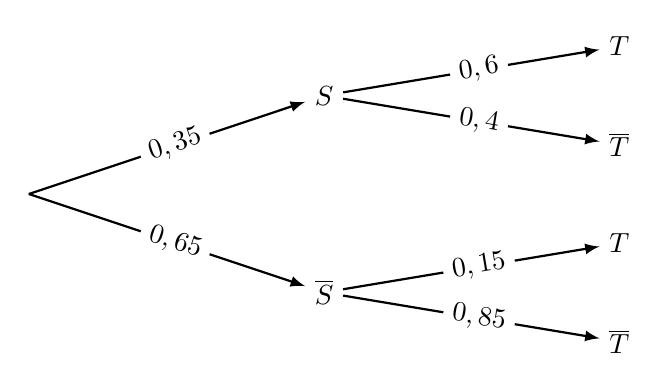
\begin{tikzpicture}
			\tikzstyle{fleche}=[->,>=latex,thick]
			\tikzstyle{noeud}=[]
			\tikzstyle{etiquette}=[sloped,pos=0.53,fill=white]
			\def\DistanceInterNiveaux{3} \def\DistanceInterFeuilles{1}
			\def\NiveauA{(0)*\DistanceInterNiveaux} \def\NiveauB{(1.25)*\DistanceInterNiveaux}
			\def\NiveauC{(2.5)*\DistanceInterNiveaux} \def\InterFeuilles{(-1.25)*\DistanceInterFeuilles}
			\coordinate (R) at ({\NiveauA},{(1.5)*\InterFeuilles}) ;
			%\node[noeud] (R) at ({\NiveauA},{(1.5)*\InterFeuilles}) {$ $};
			\node[noeud] (Ra) at ({\NiveauB},{(0.5)*\InterFeuilles}) {$S$};
			\node[noeud] (Raa) at ({\NiveauC},{(0)*\InterFeuilles}) {$T$};
			\node[noeud] (Rab) at ({\NiveauC},{(1)*\InterFeuilles}) {$\overline{T}$};
			\node[noeud] (Rb) at ({\NiveauB},{(2.5)*\InterFeuilles}) {$\overline{S}$};
			\node[noeud] (Rba) at ({\NiveauC},{(2)*\InterFeuilles}) {$T$};
			\node[noeud] (Rbb) at ({\NiveauC},{(3)*\InterFeuilles}) {$\overline{T}$};
			\draw[fleche] (R)--(Ra) node[etiquette] {$0,35$};
			\draw[fleche] (Ra)--(Raa) node[etiquette] {$0,6$};
			\draw[fleche] (Ra)--(Rab) node[etiquette] {$0,4$};
			\draw[fleche] (R)--(Rb) node[etiquette] {$0,65$};
			\draw[fleche] (Rb)--(Rba) node[etiquette] {$0,15$};
			\draw[fleche] (Rb)--(Rbb) node[etiquette] {$0,85$};
		\end{tikzpicture}
	\end{center}
	Pour chacune des affirmations suivantes, indiquer si elle est vraie ou fausse, en justifiant brièvement la réponse :
	\begin{enumerate}
		\item $p_S(T)=0,6$ ;
		\item $p(S \cap T)=0,95$ ;
		\item $p(T)=0,75$.
	\end{enumerate}
	\item Soient A et B deux évènements d'un univers $\Omega$ tels que $P(A)=0,6$ et $P(B)=0,45$ et $P(A \cap B)= 0,27$.
	\begin{enumerate}
		\item Calculer la probabilité de $A \cup B$.
		\item Les évènements A et B sont-ils indépendants ? Justifier la réponse.
	\end{enumerate}
\end{enumerate}

\bigskip

\exonum{5}

\begin{enumerate}
	\item Déterminer le tableau de signes des expressions suivantes :
	\begin{enumerate}
		\item $x^2-5x+6$ ;
		%\item $(x+2)(x^2+x+1)$ ;
		\item $\dfrac{3x-12}{0,5x^2+0,5x-1}$.
	\end{enumerate}
	\item Résoudre les inéquations suivantes :
	\begin{enumerate}
		\item $-2x^2-2x+24 > 0$ ;
		\item $(2x-3)(x^2-4x+4) \pp 0$.
	\end{enumerate}
	\item[Bonus] Résoudre l'inéquation $\dfrac{2x^2-10}{x+2} \pg -8$.
\end{enumerate}

\newpage

\exonum{4}

\medskip

Une chaîne de salons de coiffure propose à ses 5\,000 clients qui viennent pour une coupe deux prestations supplémentaires cumulables : 
\begin{itemize}
	\item une coloration naturelle à base de plantes appelée « couleur-soin »,
	\item des mèches blondes pour donner du relief à la chevelure, appelées « effet coup de soleil ». 
\end{itemize}
Il apparait que 3\,000 clients demandent une « couleur-soin ». Parmi ceux qui ne veulent pas de « couleur soin », 900 demandent un « effet coup de soleil ». Par ailleurs, 750 clients demandent une « couleur soin » et un « effet coup de soleil ». 

On notera $C$ l’évènement « le client souhaite une « couleur-soin ». 
On notera $E$ l’évènement « le client souhaite un effet coup de soleil ». 

\begin{enumerate}
	\item Compléter le tableau suivant : 
	\begin{center}
		\renewcommand{\arraystretch}{1.25}
		\setlength{\arrayrulewidth}{0.8pt}
		\begin{tabularx}{12cm}{|Y|Y|Y|Y|}
			\cline{2-4}
			\multicolumn{1}{c|}{} & C & $\overline{C}$ & Total \\ \hline
			E & & 900 & \\ \hline
			$\overline{E}$ & & & \\ \hline
			Total & & & 5\,000 \\ \hline
		\end{tabularx}
	\end{center}
	\item On interroge un client au hasard parmi les 5\,000 clients.
	\begin{enumerate}
		\item Quelle est la probabilité qu’il ait choisi les deux prestations « couleur soin » et « effet coup de soleil » ? 
		\item Quelle est la probabilité qu’il ait choisi « couleur soin » ou « effet coup de soleil » ? 
		\item Calculer $p_E \big(\overline{C}\big)$. Interpréter le résultat dans le contexte de l'exercice.
	\end{enumerate} 
\end{enumerate}

\bigskip

\exonum{7}

\medskip

Dans un magasin d’informatique, un acheteur potentiel s’intéresse à un téléphone portable et à un casque :
\begin{itemize}
	\item la probabilité pour qu’il achète le téléphone portable est $0,7$ ;
	\item la probabilité pour qu’il achète le casque quand il a acheté le téléphone portable est $0,8$ ;
	\item la probabilité pour qu’il achète le casque quand il n’a pas acheté le téléphone portable est $0,1$ 
\end{itemize}
On désigne par T l’évènement : « le client achète le téléphone portable » et par C l’évènement : « le client achète le casque ». Pour tout évènement E, on note $\overline{E}$ l’évènement contraire de E. 
\begin{enumerate}
	\item Déterminer la probabilité des évènements suivants : 
	\begin{enumerate}
		\item « Le client n'achète pas le téléphone portable » ;
		\item « Le client n'achète pas le casque sachant qu'il n’a pas acheté le téléphone portable ».
	\end{enumerate}
	\item Représenter la situation par un arbre de probabilités.
	%	
	%	Compléter l’arbre pondéré suivant : 
	%	\begin{center}
	%		\begin{tikzpicture}
	%			\tikzstyle{fleche}=[->,>=latex,thick]
	%			\tikzstyle{noeud}=[]
	%			\tikzstyle{etiquette}=[pos=0.53,sloped,fill=white]
	%			\def\DistanceInterNiveaux{3} \def\DistanceInterFeuilles{1}
	%			\def\NiveauA{(0)*\DistanceInterNiveaux} \def\NiveauB{(1.25)*\DistanceInterNiveaux}
	%			\def\NiveauC{(2.5)*\DistanceInterNiveaux} \def\InterFeuilles{(-1)*\DistanceInterFeuilles}
	%			\node[noeud] (R) at ({\NiveauA},{(1.5)*\InterFeuilles}) {$ $};
	%			\node[noeud] (Ra) at ({\NiveauB},{(0.5)*\InterFeuilles}) {$P$};
	%			\node[noeud] (Raa) at ({\NiveauC},{(0)*\InterFeuilles}) {$C$};
	%			\node[noeud] (Rab) at ({\NiveauC},{(1)*\InterFeuilles}) {$\overline{C}$};
	%			\node[noeud] (Rb) at ({\NiveauB},{(2.5)*\InterFeuilles}) {$\overline{P}$};
	%			\node[noeud] (Rba) at ({\NiveauC},{(2)*\InterFeuilles}) {$C$};
	%			\node[noeud] (Rbb) at ({\NiveauC},{(3)*\InterFeuilles}) {$\overline{C}$};
	%			\draw[fleche] (R)--(Ra) node[etiquette] {$\dots$};
	%			\draw[fleche] (Ra)--(Raa) node[etiquette] {$\dots$};
	%			\draw[fleche] (Ra)--(Rab) node[etiquette] {$\dots$};
	%			\draw[fleche] (R)--(Rb) node[etiquette] {$\dots$};
	%			\draw[fleche] (Rb)--(Rba) node[etiquette] {$\dots$};
	%			\draw[fleche] (Rb)--(Rbb) node[etiquette] {$\dots$};
	%		\end{tikzpicture}
	%	\end{center}
	\item
	\begin{enumerate}
		\item Calculer la probabilité $p(T \cap C)$. Interpréter le résultat.
		\item Déterminer la probabilité pour le client n'achète ni le téléphone portable ni le casque.
		\item Démontrer que la probabilité que l'acheteur achète un casque est de $0,59$.
		\item Sachant que le client a acheté un casque, déterminer la probabilité (arrondie au millième) qu'il ait acheté un téléphone portable.
	\end{enumerate}
	\item Les évènements T et C sont-ils indépendants ? Justifier la réponse.
\end{enumerate}

\end{document}